\documentclass[11pt]{article}
\usepackage[utf8]{inputenc}
\usepackage[T1]{fontenc}
\usepackage{geometry}
\usepackage{hyperref}
\usepackage{enumitem}
\usepackage{tikz}
\usetikzlibrary{positioning}

\geometry{margin=1in}

\title{BS Portfolio 01 MealPlanner}
\author{
  \textit{[Author Name 1]} (\textit{[Matriculation Number]})\\
  \textit{[Author Name 2]} (\textit{[Matriculation Number]})
}
\date{October 31, 2025}

\begin{document}

\maketitle

\section{Project Overview}

\textbf{Elevator Pitch.} A RESTful Meal Planner backend helps nutrition-focused users curate ingredients and dishes, then ranks meals by nutritional value per cost so they can stretch their food budgets without sacrificing protein targets.

\textbf{Why it matters.} Inflation and rising food prices make it hard for students and athletes to maintain high-protein diets. Today they juggle spreadsheets that rarely stay in sync with grocery prices. This project consolidates reliable ingredient data, automatically aggregates macro nutrients per dish, and exposes query endpoints that surface the best value choices immediately.

\textbf{Initial capabilities (MVP scope).}
\begin{itemize}[noitemsep]
  \item CRUD endpoints for ingredients recorded per 100\,g, storing name, price, protein, carbohydrates, fat, and calories.
  \item Dish management with ingredients and gram-weights, with automatic macro and cost aggregation.
  \item Read endpoints that return dishes sorted by price, protein density, calorie density, price per 100\,g protein, and price per 1000 calories via dedicated resource paths.
  \item Persistence through Quarkus with JPA, layered using hexagonal architecture (REST adapters, application services, domain core, JPA adapters).
  \item Automated testing: unit tests for aggregation rules, integration tests covering REST endpoints and database access.
\end{itemize}

\textbf{Non-goals (explicit exclusions).}
\begin{itemize}[noitemsep]
  \item Modelling allergens, sugar, salt, or micronutrients in MVP (left for a future iteration).
  \item Personal accounts, authentication, or company-specific branding.
  \item Recipe recommendation engines or meal-plan generation---focus stays on ranking and manual selection.
\end{itemize}

\section{Domain Model}

The core entities and relationships are illustrated in Figure~\ref{fig:uml}. The domain enforces that dishes contain at least one ingredient and each ingredient line stores a gram quantity to derive totals.

\begin{figure}[h]
  \centering
  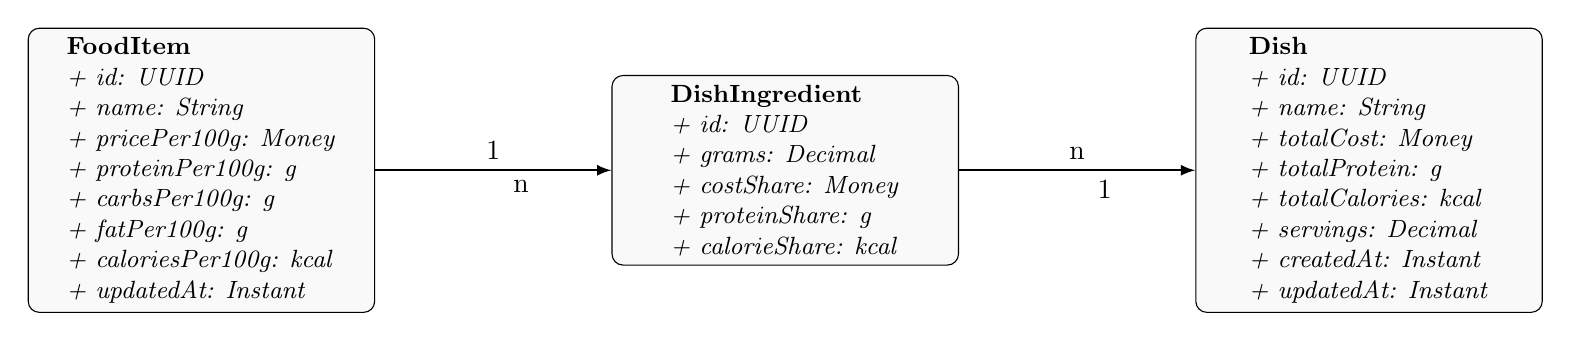
\begin{tikzpicture}[
    class/.style={rectangle, draw, rounded corners, minimum width=4.4cm, align=left, font=\small, fill=gray!5},
    relation/.style={-latex, thick},
    node distance=3.0cm
  ]

    \node[class] (food) {
      \textbf{FoodItem}\\
      \textit{+ id: UUID}\\
      \textit{+ name: String}\\
      \textit{+ pricePer100g: Money}\\
      \textit{+ proteinPer100g: g}\\
      \textit{+ carbsPer100g: g}\\
      \textit{+ fatPer100g: g}\\
      \textit{+ caloriesPer100g: kcal}\\
      \textit{+ updatedAt: Instant}
    };

    \node[class, right=of food] (dishIng) {
      \textbf{DishIngredient}\\
      \textit{+ id: UUID}\\
      \textit{+ grams: Decimal}\\
      \textit{+ costShare: Money}\\
      \textit{+ proteinShare: g}\\
      \textit{+ calorieShare: kcal}
    };

    \node[class, right=of dishIng] (dish) {
      \textbf{Dish}\\
      \textit{+ id: UUID}\\
      \textit{+ name: String}\\
      \textit{+ totalCost: Money}\\
      \textit{+ totalProtein: g}\\
      \textit{+ totalCalories: kcal}\\
      \textit{+ servings: Decimal}\\
      \textit{+ createdAt: Instant}\\
      \textit{+ updatedAt: Instant}
    };

    \draw[relation] (food) -- node[above]{1} node[below]{\quad\quad n} (dishIng);
    \draw[relation] (dishIng) -- node[above]{n} node[below]{\quad\quad 1} (dish);
  \end{tikzpicture}
  \caption{UML class diagram of the Meal Planner domain.}
  \label{fig:uml}
\end{figure}

\paragraph{Key entities.} \textbf{FoodItem} stores the canonical nutritional facts per 100\,g and current market price. \textbf{Dish} aggregates one or more \textbf{DishIngredient} records, which capture how much of each ingredient is used along with denormalised totals (ensuring quick read performance when sorting). Totals are recalculated in the domain layer whenever a dish changes.

\paragraph{Example records.}
\begin{itemize}[noitemsep]
  \item FoodItem: \emph{``Chicken Breast''}, price 1{,}89\,€ / 100\,g, protein 23\,g, carbs 0\,g, fat 1{,}5\,g, calories 110\,kcal.
  \item Dish: \emph{``Budget Protein Bowl''} with ingredients (150\,g Chicken Breast, 100\,g Rice, 50\,g Broccoli) resulting in total cost 2{,}45\,€, total protein 38\,g, total calories 510\,kcal.
\end{itemize}

\section{Use Cases}

The project will support the following core use cases. Each includes priority (Must/Should/Could), preconditions, main success path, failure flows, postconditions, and acceptance criteria.

\subsection*{UC01 -- Register Food Item (Must)}
\textbf{Primary Actor:} Data curator.\\
\textbf{Goal (User Story):} ``As a curator I want to register a base ingredient with macro values and price so the system can use the data in dishes.''\\
\textbf{Preconditions:} Ingredient name is unique; mandatory macro and price fields provided.\\
\textbf{Main Success Scenario:}
\begin{enumerate}[label=\arabic*.]
  \item Actor sends \texttt{POST /food-items} with name, macros per 100\,g, price, and timestamp.
  \item System validates ranges (e.g., no negative macros).
  \item System persists FoodItem via JPA repository.
  \item API returns \texttt{201 Created} with generated ID.
\end{enumerate}
\textbf{Alternate / Failure Flows:}
\begin{enumerate}[label=\arabic*F.]
  \item Duplicate name detected $\rightarrow$ respond \texttt{409 Conflict}.
  \item Validation error (e.g., missing protein) $\rightarrow$ respond \texttt{400 Bad Request}.
\end{enumerate}
\textbf{Postconditions:} FoodItem stored and available for dish composition.\\
\textbf{Acceptance Criteria:}
\begin{itemize}[noitemsep]
  \item Numeric values up to two decimals; negative submissions rejected.
  \item Unit tests cover validation boundaries.
\end{itemize}

\subsection*{UC02 -- Compose Dish (Must)}
\textbf{Primary Actor:} Nutritional planner.\\
\textbf{Goal (User Story):} ``As a planner I want to assemble a dish from specific ingredient weights so totals update automatically.''\\
\textbf{Preconditions:} At least one FoodItem exists.\\
\textbf{Main Success Scenario:}
\begin{enumerate}[label=\arabic*.]
  \item Actor calls \texttt{POST /dishes} with name, servings, and ingredient list (\texttt{foodItemId}, grams).
  \item System loads referenced FoodItems.
  \item Domain service calculates aggregated macros, cost, and per-serving metrics.
  \item Dish plus DishIngredient entities persist inside a transaction.
  \item API returns \texttt{201 Created} with calculated totals.
\end{enumerate}
\textbf{Alternate / Failure Flows:}
\begin{enumerate}[label=\arabic*F.]
  \item Unknown FoodItem ID $\rightarrow$ \texttt{404 Not Found}.
  \item Ingredient grams $\leq 0$ $\rightarrow$ \texttt{400 Bad Request}.
\end{enumerate}
\textbf{Postconditions:} Dish totals reflect submitted ingredients.\\
\textbf{Acceptance Criteria:}
\begin{itemize}[noitemsep]
  \item Totals equal sum of ingredient contributions within rounding tolerance.
  \item Integration test verifies persistence and retrieval reproduces totals.
\end{itemize}

\subsection*{UC03 -- Adjust Dish Composition (Should)}
\textbf{Primary Actor:} Nutritional planner.\\
\textbf{Goal (User Story):} ``As a planner I want to update ingredient weights so cost-per-protein stays accurate.''\\
\textbf{Preconditions:} Dish exists with at least one ingredient.\\
\textbf{Main Success Scenario:}
\begin{enumerate}[label=\arabic*.]
  \item Actor issues \texttt{PUT /dishes/\{dishId\}} with modified ingredient list.
  \item System reapplies domain rules to recompute totals and price metrics.
  \item Transaction persists new DishIngredient rows, removing obsolete ones.
  \item API returns updated DTO with timestamps.
\end{enumerate}
\textbf{Alternate / Failure Flows:}
\begin{enumerate}[label=\arabic*F.]
  \item Dish locked by another transaction $\rightarrow$ respond \texttt{409 Conflict}.
  \item Removal of all ingredients $\rightarrow$ reject with \texttt{400}, message ``Dish must contain at least one ingredient.''
\end{enumerate}
\textbf{Postconditions:} Dish reflects new macro and cost totals.\\
\textbf{Acceptance Criteria:}
\begin{itemize}[noitemsep]
  \item Integration tests ensure per-serving calculations update after change.
  \item Optimistic locking guards against concurrent overwrites.
\end{itemize}

\subsection*{UC04 -- Retrieve Ranked Dishes (Must)}
\textbf{Primary Actor:} Shopper preparing meal plans.\\
\textbf{Goal (User Story):} ``As a shopper I want to list dishes sorted by specific value so I can pick the most cost-effective meals.''\\
\textbf{Preconditions:} At least one dish exists with aggregated metrics.\\
\textbf{Main Success Scenario:}
\begin{enumerate}[label=\arabic*.]
  \item Actor calls dedicated endpoints such as:
  \begin{itemize}[noitemsep]
    \item \texttt{GET /dishes/sorted-by-price}
    \item \texttt{GET /dishes/sorted-by-protein}
    \item \texttt{GET /dishes/sorted-by-calories}
    \item \texttt{GET /dishes/sorted-by-price-per-protein}
    \item \texttt{GET /dishes/sorted-by-price-per-calorie}
  \end{itemize}
  \item Application service queries database with appropriate \texttt{ORDER BY}.
  \item Results return as paginated JSON list including ranks and summary metrics.
\end{enumerate}
\textbf{Alternate / Failure Flows:}
\begin{enumerate}[label=\arabic*F.]
  \item No dishes found $\rightarrow$ respond \texttt{200} with empty array.
  \item Unsupported sort path requested $\rightarrow$ \texttt{404 Not Found}.
\end{enumerate}
\textbf{Postconditions:} User receives ordered dish list for immediate comparison.\\
\textbf{Acceptance Criteria:}
\begin{itemize}[noitemsep]
  \item Sorting stable for dishes with equal metric values.
  \item Integration tests assert ordering correctness for each endpoint.
\end{itemize}

\subsection*{UC05 -- Inspect Ingredient Impact (Could)}
\textbf{Primary Actor:} Planner evaluating substitutions.\\
\textbf{Goal (User Story):} ``As a planner I want to see how a FoodItem contributes to total dish cost and macros so I can replace expensive ingredients.''\\
\textbf{Preconditions:} Dish with recorded DishIngredients.\\
\textbf{Main Success Scenario:}
\begin{enumerate}[label=\arabic*.]
  \item Actor calls \texttt{GET /dishes/\{dishId\}/ingredients/\{ingredientId\}}.
  \item System returns macro and cost share percentages.
\end{enumerate}
\textbf{Alternate / Failure Flows:}
\begin{enumerate}[label=\arabic*F.]
  \item Ingredient not present in dish $\rightarrow$ \texttt{404 Not Found}.
\end{enumerate}
\textbf{Postconditions:} Planner sees how each ingredient contributes.\\
\textbf{Acceptance Criteria:}
\begin{itemize}[noitemsep]
  \item Percentages sum to 100\% across all ingredients (within rounding tolerance).
  \item Endpoint disabled in MVP if time constraints demand---marked Could.
\end{itemize}

\section{Testing and Quality Approach}

\begin{itemize}[noitemsep]
  \item \textbf{Unit tests} target domain services: macro aggregation, price-per-metric calculations, validation rules.
  \item \textbf{Integration tests} spin up Quarkus with an in-memory database to cover REST endpoints, JPA repositories, and JSON contracts.
  \item \textbf{Contract checks} ensure DTOs remain backward compatible when new fields (e.g., micronutrients) are added later.
  \item \textbf{Continuous Integration} enforces formatting, static analysis, and test execution to maintain a releasable trunk.
\end{itemize}

\end{document}
